\documentclass[12pt,a4paper,hidelinks,english]{report}
\usepackage[utf8]{inputenc}
\usepackage{amsmath}
\usepackage{booktabs}
\usepackage{caption}
\captionsetup{justification=centering,font=footnotesize}
\usepackage[nooldvoltagedirection]{circuitikz}
\usepackage[english]{babel}
\usepackage[style=alphabetic]{biblatex}
\addbibresource{references.bib}
\usepackage[margin=2.5cm]{geometry}
\usepackage{graphicx}
\graphicspath{{images/}}
\usepackage{hyperref}
\usepackage{ifthen}
\usepackage{pgfplots}
\pgfplotsset{width=9cm,compat=1.10}
\usepackage{pythontex}
\setpythontexoutputdir{.}
\usepackage[english=american]{csquotes}
\usepackage[binary-units=true]{siunitx}
\sisetup{locale = US}
\usepackage{tabularx}
\usepackage{tocbibind}
\usepackage{fancyhdr}
\pagestyle{fancy}
\fancyhead{}
\fancyhead[L]{\leftmark}
\fancyfoot{}
\fancyfoot[C]{\thepage}
\setlength{\headheight}{15pt}
\renewcommand{\chaptermark}[1]{\markboth{\chaptername{} \ \thechapter.\ #1}{}}
\usepackage{tikz}
\usetikzlibrary{intersections,matrix,positioning}

\title{Developer Manual: Digital Clock \\
\large for Computer Architecture Course at University of Esslingen}
\author{Andreas Baulig \and Jakob Janusch}
\date{May 2020}

\begin{document}

\maketitle{}

\tableofcontents

\listoffigures

% !TeX root = ../main.tex
\chapter{Introduction}

Purpose of this document is to describe and explain the inner workings of the digital clock application, created as part of lab exercise 4.1 in the Computer Architecture course at the University of Esslingen.

A description of operation, functional and non-functional requirements; as well as design requirements are described in the lab exercise sheet. This document will focus on \emph{how} things are implemented, not \emph{why}.

The manual is structured in chapters, each describing an individual module. A module description consists of the public interface, used to interact with other modules; as well as implementation details.

\section{Module Overview}\label{sec:module_overview}

Figure \ref{fig:module_overview} depicts a logical component view of the entire application.

Component \emph{Main Loop} sits atop the structure and is responsible for sequencing the application flow. It itself is timed and driven by the \emph{Tick Generator} interface, provided by the \emph{Wrapper} subsystem. The generated tick is at a higher frequency than what is needed for most of the other components, so \emph{Main Loop} divides the incoming \emph{Short Tick} into an additional \emph{Long Tick}.

All user interaction is controlled through the \emph{User Interface} (abbr.\ UI) component. This includes:
\begin{itemize}
    \item Buttons
    \item LCD
    \item LEDs
\end{itemize}
It also controls the operating modes, such as SET-mode and NORMAL-mode.

The UI component requires both, Short and Long Tick, to facilitate all its functions, while all other components work on Long Tick alone.

The overall timekeeping functionality is provided by the \emph{Clock} component. It consumes a Long Tick, that is used to increment the internal seconds, minutes and hours counters. The current time can then be read out through its \emph{Current Time} interface.

Temperature measurements are performed by a dedicated component called \emph{Thermometer}. It enables measurements of the internal ADC, does the necessary conversion and provides the value via \emph{Get Last Measurement}. Taking measurements is also driven by Long Tick, and is done at the start of each new Long Tick update cycle.

Lastly the \emph{Wrapper} subsystem provides miscellaneous interfaces such as driving the LCD and converting \SI{16}{\bit} integers to decimal formatted ASCII strings. These functions are implemented in HCS12 Assembly and do not follow standard C call-convention, which is why wrapping is needed to facilitate safe C/Assembly inter-operation.

\begin{figure}[ht]
    \centering
    \includegraphics[width=\textwidth]{generated/components.png}
    \caption{Module Overview}\label{fig:module_overview}
\end{figure}

% !TeX root = ../main.tex
\chapter{User Interface}

\section{Objectives}

\begin{itemize}
    \item Control LCD output of current time, temperature and info text.
    \item Poll button press and held events.
    \item Switch operating mode depending on button events and current state information.
    \item Drive LEDs depending on current state information.
\end{itemize}

\section{Interface}

\begin{itemize}
    \item Initialize
          \begin{itemize}
              \item Initialize the state information and required sub-modules, such as the LCD driver, LED and push-button pin-modes.
          \end{itemize}
    \item Short Tick (\(f_{S}=\SI{100}{\hertz}\))
          \begin{itemize}
              \item Debounce push buttons.
              \item Recognize press and held events depending on current operating mode.
          \end{itemize}
    \item Long Tick (\(f_{L}=\SI{1}{\hertz}\))
          \begin{itemize}
              \item Update time and temperature display on LCD.
              \item Toggle LED 0 with each tick.
              \item Subdivide Long Tick further to switch info text display every \SI{5}{\second}.
          \end{itemize}
\end{itemize}

\section{Details}

\subsection{Short Tick vs. Long Tick}

The use of Short Tick to control button handing versus Long Tick is based on the need for low latency press and held event detection. Polling button states on Long Tick would increase latency to up to \SI{1}{\second}, before the press is even detected. Held events could subsequently also only be detected on increments of \SI{1}{\second}, leading to an overall sluggish interaction/feedback cycle.

With a frequency of \SI{100}{\hertz}, Short Tick provides a good time-basis to perform acceptable in-software button debouncing, while maintaining high reactance to even very short user inputs.

To avoid confusion, tick counters are marked either by naming or in-code Doxygen documentation, as to which tick domain they belong to.

\subsection{Button Events}

Button states are checked on every Short Tick. Which specific buttons are checked, depends on the current operating mode. Button events can be categorized either as press or held events. The method of detecting the \emph{start-of-event} is the same for both categories, and involves comparing the current button state to the state from the last tick. If the button state switched from released to pushed, that tick is saved as start-of-event.

\subsubsection{Press Events}

A \emph{press} is detected, if the button is pushed and held for a specified number of ticks, called \texttt{ticks\_to\_activate}. The corresponding event is raised once, and the button is put on \emph{cool-down}. In this state, no further press events will be raised for this button. Cool-down ends when the button is released again, enabling the user to perform the next press event.

Figure~\ref{fig:press_events} an exemplary snipped from an impulse diagram. In the shown graph \(\texttt{ticks\_to\_activate} = 1\), resulting in button pushes shorter than that to be ignored. If the button is held down longer than \texttt{ticks\_to\_activate}, a single pressed event is raised.

\begin{figure}
    \centering

    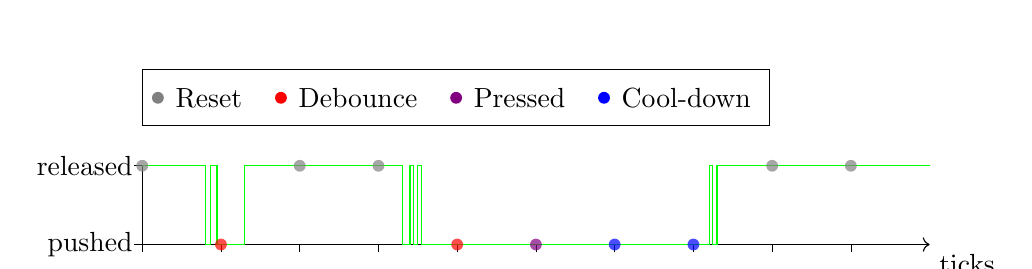
\begin{tikzpicture}
        \draw [very thin] (-0.1,0) -- (0,0) (-0.1,1) -- (0,1);
        \foreach \x in {0,...,9}
            {
                \draw [very thin] (\x,-0.1) -- (\x,0);
                \path [name path=ticks\x] (\x,0) -- (\x,1);
            }

        \draw [->] (0,0) -- (10,0) node [anchor=north west] {ticks};
        \draw (0,0) -- (0,1) node [anchor=east,at end] {released} node [anchor=east,at start] {pushed};

        \draw [name path=button,green] (0,1) -- (0.8,1) -- (0.8,0) -- (0.87,0) -- (0.87,1) -- (0.95,1) -- (0.95,0) -- (1.3,0) -- (1.3,1) -- (3.3,1) -- (3.3,0) -- (3.4,0) -- (3.4,1) -- (3.44,1) -- (3.44,0) -- (3.5,0) -- (3.5,1) -- (3.55,1) -- (3.55,0) -- (7.2,0) -- (7.2,1) -- (7.24,1) -- (7.24,0) -- (7.3,0) -- (7.3,1) -- (10,1);


        \newcounter{tickspushedpress}

        \foreach \x in {0,...,9}
            {
                \fill [opacity=0.7, name intersections={of=button and ticks\x,by=curr}]
                (curr) circle (0.075)
                let \p1=(curr) in \pgfextra{
                    \ifthenelse{1>\y1}{
                        \stepcounter{tickspushedpress}
                        \ifthenelse{\thetickspushedpress<2}{
                            \def\intersectcolor{red}
                        }{
                            \ifthenelse{\thetickspushedpress=2}{
                                \def\intersectcolor{violet}
                            }{
                                \def\intersectcolor{blue}
                            }
                        }
                    }{
                        \setcounter{tickspushedpress}{0}
                        \def\intersectcolor{gray}
                    }
                } [color=\intersectcolor];
            }

        \coordinate (top) at (0,1);
        \matrix [matrix of nodes,draw,above right=0.5 and 0 of top,column sep=0.3cm]
        {
            \fill [color=gray] (0,0) circle (0.075) node [xshift=0.1cm,color=black,anchor=west] {Reset}; &
            \fill [color=red] (0,0) circle (0.075) node [xshift=0.1cm,color=black,anchor=west] {Debounce}; &
            \fill [color=violet] (0,0) circle (0.075) node [xshift=0.1cm,color=black,anchor=west] {Pressed}; &
            \fill [color=blue] (0,0) circle (0.075) node [xshift=0.1cm,color=black,anchor=west] {Cool-down};   \\
        };

    \end{tikzpicture}
    \caption{Press Events}\label{fig:press_events}
\end{figure}

\subsubsection{Held Events}\label{sec:held_events}

Similar to press events, \emph{held} events also involve a minimum specified number of ticks to activate, called \texttt{ticks\_to\_activate}. After first activation, the button is put on \emph{cool-down}. Conversely to \emph{press} events however, cool-down ends after a second specified number of ticks have passed since activation, called \texttt{ticks\_to\_reactivate}. The time of last activation is then updated to the current tick count and a new reactivation timeout begins. This process continues as long as the button is being pushed down. The frequency of held events can be controlled through \texttt{ticks\_to\_reactivate}, while \texttt{ticks\_to\_activate} controls how long the button has to be pushed initially before the first held event is raised.

The example in figure~\ref{fig:held_events} shows a set up with \(\texttt{ticks\_to\_activate} = 2\) and \(\texttt{\_reactivate} = 1\). It can be seen, that the initial held event is delayed. Subsequent held events on the other hand, are fired in shorter intervals.

\begin{figure}
    \centering

    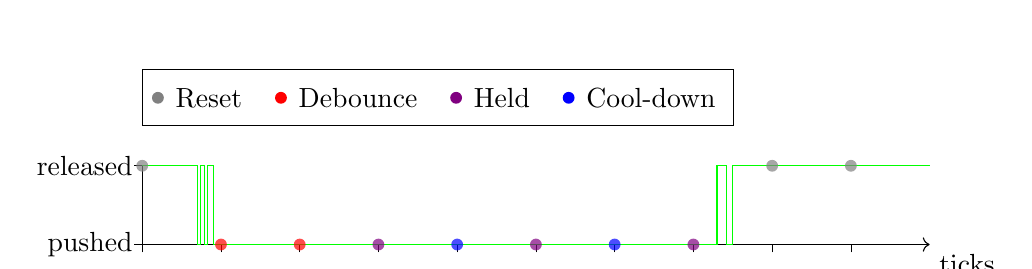
\begin{tikzpicture}
        \draw [very thin] (-0.1,0) -- (0,0) (-0.1,1) -- (0,1);
        \foreach \x in {0,...,9}
            {
                \draw [very thin] (\x,-0.1) -- (\x,0);
                \path [name path=ticks\x] (\x,0) -- (\x,1);
            }

        \draw [->] (0,0) -- (10,0) node [anchor=north west] {ticks};
        \draw (0,0) -- (0,1) node [anchor=east,at end] {released} node [anchor=east,at start] {pushed};


        \draw [name path=button,green] (0,1) -- (0.7,1) -- (0.7,0) -- (0.74,0) -- (0.74,1) -- (0.79,1) -- (0.79,0) -- (0.83,0) -- (0.83,1) -- (0.91,1) -- (0.91,0) -- (7.3,0) -- (7.3,1) -- (7.34,1) -- (7.42,1) -- (7.42,0) -- (7.5,0) -- (7.5,1) -- (10,1);


        \newcounter{tickspushedheld}
        \newcounter{tickspushedcooldown}

        \foreach \x in {0,...,9}
            {
                \fill [opacity=0.7, name intersections={of=button and ticks\x,by=curr}]
                (curr) circle (0.075)
                let \p1=(curr) in \pgfextra{
                    \ifthenelse{1>\y1}{
                        \stepcounter{tickspushedheld}
                        \ifthenelse{\thetickspushedheld<3}{
                            \def\intersectcolor{red}
                        }{
                            \ifthenelse{\thetickspushedheld=3}{
                                \def\intersectcolor{violet}
                            }{
                                \def\intersectcolor{blue}
                                \stepcounter{tickspushedcooldown}
                                \ifthenelse{\thetickspushedcooldown=1}{
                                    \setcounter{tickspushedheld}{2}
                                    \setcounter{tickspushedcooldown}{0}
                                }{}
                            }
                        }
                    }{
                        \setcounter{tickspushedheld}{0}
                        \setcounter{tickspushedcooldown}{0}
                        \def\intersectcolor{gray}
                    }
                } [color=\intersectcolor];
            }

        \coordinate (top) at (0,1);
        \matrix [matrix of nodes,draw,above right=0.5 and 0 of top,column sep=0.3cm]
        {
            \fill [color=gray] (0,0) circle (0.075) node [xshift=0.1cm,color=black,anchor=west] {Reset};  &
            \fill [color=red] (0,0) circle (0.075) node [xshift=0.1cm,color=black,anchor=west] {Debounce}; &
            \fill [color=violet] (0,0) circle (0.075) node [xshift=0.1cm,color=black,anchor=west] {Held}; &
            \fill [color=blue] (0,0) circle (0.075) node [xshift=0.1cm,color=black,anchor=west] {Cool-down};   \\
        };

    \end{tikzpicture}
    \caption{Held Events}\label{fig:held_events}
\end{figure}

\subsection{Modes of Operation}

\subsubsection{NORMAL-Mode}

On boot-up NORMAL-mode is entered. In this mode time and temperature are updated with every Long Tick. Time is obtained from the Clock module, while the value for temperature is taken from the Thermometer's last measured value.

Pressing the \texttt{SWITCH\_MODE\_BUTTON} for more than \texttt{LONG\_PRESS\_SHORT\_TICK\_COUNT}, will result in a switch to SET-Mode.

\subsubsection{SET-Mode}

While in SET-mode, pressing the \texttt{INCREMENT\_SECONDS\_}, \texttt{\_MINUTES\_} or \texttt{\_HOURS\_BUTTON}, will increment the Clock modules current seconds, minutes or hours setting respectively. Note that incrementing these values makes use of the button held events discussed in section~\ref{sec:held_events}, allowing for precise single-step and fast multi-step changes.
When changing the time, the updated values are displayed immediately. Relying on Long Tick would lead to a perceived high latency when changing time, with multiple increments happening within the same Long Tick.

SET-mode can be exited the same way it was entered, by pressing \texttt{SWITCH\_MODE\_BUTTON} for \texttt{SHORT\_PRESS\_SHORT\_TICK\_COUNT}.

\subsection{Display}

The LCD is split into two lines, the upper one displays the current time and temperature and is updated each Long Tick. The lower one switches between displaying the copyright information and names of the authors. Switching between copyright and names is done every \SI{5}{\second} using a tick counter based on Long Tick. Note that during SET-mode, time is updated immediately upon changing the Clock settings.

With every Long Tick, LED on pin 0 is toggled.

% !TeX root = ../main.tex
\chapter{The Clock Module}

\section{Objectives}

\begin{itemize}
    \item Store system date and time as components of Gregorian calendar:
          \begin{itemize}
              \item Seconds (\numrange{0}{59})
              \item Minutes (\numrange{0}{59})
              \item Hours (\numrange{0}{23})
              \item Days in month (\numrange{1}{31}, \numrange{1}{30}, \numrange{1}{29} or \numrange{1}{28} depending on month and year; \num{0} it to be considered invalid)
              \item Day of week (\numrange{1}{7} representing days Monday to Sunday; \num{0} is to be considered invalid)
              \item Months (\numrange{1}{12}; \num{0} it to be considered invalid)
              \item Years (starting at year \num{1})
          \end{itemize}
    \item Increment seconds counter every second.
    \item Allow user to switch timezone via button press.
    \item Single point of access to LCD display of date and time.
\end{itemize}

\section{Interface}

\begin{itemize}
    \item House sys-tick, used to increment second counter and do other housekeeping stuff.
    \item Process \emph{second passed} events through non-ISR function.
    \item Set system date and time.
\end{itemize}

\section{Details}

\subsection{Determining Day of Week}\label{sec:determining_day_of_week}

While the DCF77 frame does contain a distinct field for day-of-week, the Gregorian calendar date alone is sufficient to determine this information already. The algorithm to do so is fairly compact and doesn't require very much calculating. It is based on the fact that certain months start on the same day-of-week \cite{Mishra2016} and \DTMenglishmonthname{1} \nth{1} of year 0001 is set on a Monday. There are of course complications, as the number of days per year vary from \numrange{365}{366}, depending on the type of year. Years with \num{366} days are referred to as \emph{leap years}, while years with \num{365} days are considered \emph{normal years}. An algorithm to determine whether a given year is a leap or normal year is depicted in Figure~\ref{fig:leap_year}.

\begin{figure}
    \centering
    \includeinkscape[width=\textwidth]{generated/leap_year.pdf_tex}
    \caption{Algorithm to determine whether a given year is a leap or normal year.}\label{fig:leap_year}
\end{figure}

The way the algorithm accounts for these additional days (called \emph{leap days}) is by first calculating the total number of leap days for a given year since year \num{1}. Taking the remainder of the sum of all leap days plus the year value results in the day-of-week for \DTMenglishmonthname{1} \nth{1} of that year (see Equation~\ref{equ:january_first_of_year}).

\begin{equation}\label{equ:january_first_of_year}
    \text{day-of-week}_{\text{Jan \nth{1}}}(y) = \left(y + \lfloor y/4 \rfloor - \lfloor y/100 \rfloor + \lfloor y/400 \rfloor\right) \mod{7}
\end{equation}

Utilizing the insight that certain months start on the same day-of-week, a look-up table (as depicted in Column \emph{Normal Offset} of Table~\ref{tab:start_of_months_offsets}) with offsets relative to \DTMenglishmonthname{1} \nth{1} can be generated.

\begin{table}[htb]
    \centering
    \begin{tabularx}{0.55\textwidth}{r c c}
        \toprule
        Month                    & Normal Offset & Corrected Offset \\
        \midrule
        \DTMenglishmonthname{1}  & \num{0}       & \num{0}          \\
        \DTMenglishmonthname{2}  & \num{3}       & \num{3}          \\
        \DTMenglishmonthname{3}  & \num{3}       & \num{2}          \\
        \DTMenglishmonthname{4}  & \num{6}       & \num{5}          \\
        \DTMenglishmonthname{5}  & \num{1}       & \num{0}          \\
        \DTMenglishmonthname{6}  & \num{4}       & \num{3}          \\
        \DTMenglishmonthname{7}  & \num{6}       & \num{5}          \\
        \DTMenglishmonthname{8}  & \num{2}       & \num{1}          \\
        \DTMenglishmonthname{9}  & \num{5}       & \num{4}          \\
        \DTMenglishmonthname{10} & \num{0}       & \num{6}          \\
        \DTMenglishmonthname{11} & \num{3}       & \num{2}          \\
        \DTMenglishmonthname{12} & \num{5}       & \num{4}          \\
        \bottomrule
    \end{tabularx}
    \caption{Look-up table with start-of-month offsets relative to \DTMenglishmonthname{1} \nth{1}.}\label{tab:start_of_months_offsets}
\end{table}

However, before a look-up can be made, the current month needs to be taken into consideration. Leap days in the Gregorian system are only applied at the end of month \DTMenglishmonthname{2}, not \DTMenglishmonthname{1}, as Equation~\ref{equ:january_first_of_year} assumes. This can be fixed by subtracting the year count by one before calculating the number of leap days, if the month in question is \DTMenglishmonthname{3} or beyond. To fix the now resulting off-by-one-error for months \DTMenglishmonthname{3} to \DTMenglishmonthname{12}, in cases where the leap day for the current year was dropped, a modified look-up table can be generated. This table decrements each offset by one, starting with the month of \DTMenglishmonthname{3} (see Column \emph{Corrected Offset} of Table~\ref{tab:start_of_months_offsets}).

\subsection{Handling Date Over-/Underflows}

A date over- or underflow happens, when one component of the date/time structure wraps around and in-/decrements the next one. A simple example where this might happen is every day at \DTMdisplaytime{23}{59}{59}. The next second will be \DTMdisplaytime{00}{00}{00} of the following day. If the day counter already sits at the end-of-month, months need to be incremented as well. Same applies for the month of \DTMenglishmonthname{12}, after which the year counter needs to be incremented.

The way this mechanism is implemented in the embedded application is by singular increment or decrement functions for each date/time component. If an over-/underflow is detected, the next date/time component is updated and so on. Offsetting the date/time structure by multiple steps (as for handling timezones) is done by in-/decrementing the corresponding field multiple times until the desired offset is reached. After each change of date, the day-of-week is calculated anew, using the algorithm discussed in Section~\ref{sec:determining_day_of_week}.

\subsection{Timezones}

Two timezones are supported: DCF77 or DE (\num[explicit-sign=+]{0}) and US (\num{-6}). Note that daylight-saving-time is not accounted for, and the offset caused by it remains unchanged.

Switching timezones is done via press of button \texttt{H.3}. Button debouncing and handling is implemented directly inside the Clock module, by polling the button state inside the \SI{10}{\milli\second} tick interrupt.

The timezone offset is applied only on the display output. The internal representation of the date/time remains unchanged and always assumes DCF77 (or German) time.


\end{document}
